\documentclass[tikz,border=3pt]{standalone}
\usepackage[utf8]{inputenc}
\usepackage[T1]{fontenc}
\usepackage{libertinus}
\usepackage{amsmath,amssymb}
\usepackage{pgfplots}
\pgfplotsset{compat=1.18}
\usetikzlibrary{arrows.meta}
\definecolor{UGblue}{RGB}{0,51,102}
\begin{document}
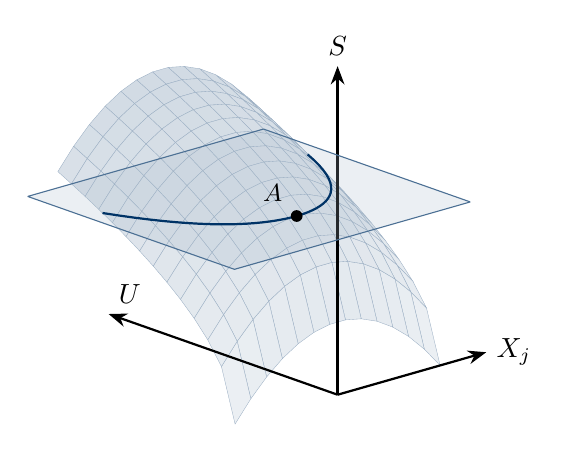
\begin{tikzpicture}
\begin{axis}[hide axis,view={-42}{22},width=9.5cm,height=8.5cm,xmin=-1.6,xmax=1.6,ymin=-0.3,ymax=1.7,zmin=0,zmax=1.9,z buffer=sort,clip=false,>=Stealth,
  colormap={s}{color(0cm)=(UGblue!6) color(1cm)=(UGblue!18)}]
\addplot3[surf,shader=flat,draw=UGblue!40,line width=0.12pt,domain=0:1.2,y domain=-1:1,samples=14,samples y=14,z buffer=sort]
  ({y},{x},{0.4+0.95*sqrt(x)-0.4*y*y});
\draw[->,thick] (axis cs:0,0,0) -- (axis cs:1.45,0,0) node[right] {$X_j$};
\draw[->,thick] (axis cs:0,0,0) -- (axis cs:0,1.55,0) node[above right] {$U$};
\draw[->,thick] (axis cs:0,0,0) -- (axis cs:0,0,1.8) node[above] {$S$};
\addplot3[patch,patch type=rectangle,shader=flat,fill=UGblue!35,fill opacity=0.22,draw=UGblue!70,line width=0.4pt] coordinates {(-1.15,-0.1,0.9) (1.15,-0.1,0.9) (1.15,1.3,0.9) (-1.15,1.3,0.9)};
\draw[thick,UGblue] plot[domain=-1:1,samples=40,variable=\t] (axis cs:{\t},{((0.5+0.4*\t*\t)/0.95)^2},{0.9});
\node[circle,fill,inner sep=1.5pt,label={[font=\small]above left:$A$}] at (axis cs:0.0000,0.2770,0.9000) {};
\end{axis}
\end{tikzpicture}
\end{document}
